\documentclass[11pt,a4paper]{article}
\usepackage[utf8]{inputenc}
\usepackage[T1]{fontenc}
\usepackage{lmodern}
\usepackage[portuguese]{babel}
\usepackage[a4paper,margin=2.4cm]{geometry}
\usepackage{xcolor}
\usepackage{graphicx}
\usepackage{titlesec}
\usepackage{enumitem}
\usepackage{listings}
\usepackage{tcolorbox}
\usepackage{booktabs}
\usepackage{amsmath}
\usepackage{amssymb}
\usepackage{fancyhdr}
\usepackage{hyperref}
\tcbuselibrary{skins,breakable,listings}

\definecolor{BgCream}{HTML}{FAF8F5}
\definecolor{TextEspresso}{HTML}{4A4238}
\definecolor{NudeTaupe}{HTML}{BFAFA6}
\definecolor{SoftBlush}{HTML}{D9C5B2}
\definecolor{SageMuted}{HTML}{7E8F7C}
\definecolor{ClayWarn}{HTML}{B5795C}

\hypersetup{colorlinks=true, linkcolor=TextEspresso, urlcolor=TextEspresso}

\titleformat{\section}{\color{TextEspresso}\Large\bfseries}{\thesection}{0.6em}{}[{\color{NudeTaupe}\titlerule[0.8pt]}]
\titleformat{\subsection}{\color{TextEspresso}\large\bfseries}{\thesubsection}{0.6em}{}
\titlespacing*{\section}{0pt}{1.4\baselineskip}{0.7\baselineskip}
\titlespacing*{\subsection}{0pt}{1.1\baselineskip}{0.5\baselineskip}

\lstset{
  basicstyle=\ttfamily\small,
  breaklines=true,
  columns=fullflexible,
  showstringspaces=false,
  frame=none,
  aboveskip=0pt, belowskip=0pt
}

\pagestyle{fancy}
\fancyhf{}
\renewcommand{\headrulewidth}{0pt}
\fancyfoot[C]{\color{NudeTaupe}\small\thepage}

% ---- Caixa: comandos a executar ----
\newtcblisting{terminal}{
  listing only, breakable,
  colback=BgCream, colframe=NudeTaupe,
  boxrule=0.5pt, arc=2pt, left=6pt, right=6pt, top=5pt, bottom=5pt,
  listing options={basicstyle=\ttfamily\small, breaklines=true, columns=fullflexible}
}

% ---- Caixa: saida esperada ----
\newtcblisting{saida}{
  listing only, breakable,
  colback=white, colframe=SoftBlush,
  boxrule=0.5pt, arc=2pt, left=6pt, right=6pt, top=5pt, bottom=5pt,
  title={\small\bfseries\color{TextEspresso}Saída esperada},
  coltitle=TextEspresso, colbacktitle=SoftBlush!45,
  fonttitle=\small\bfseries,
  listing options={basicstyle=\ttfamily\footnotesize, breaklines=true, columns=fullflexible}
}

% ---- Caixa: ponto de verificacao ----
\newtcolorbox{verificar}{
  breakable, colback=SageMuted!8, colframe=SageMuted,
  boxrule=0.6pt, arc=2pt, left=7pt, right=7pt, top=6pt, bottom=6pt,
  title={\small\bfseries Confirme antes de avançar},
  coltitle=white, colbacktitle=SageMuted, fonttitle=\small\bfseries
}

% ---- Caixa: aviso ----
\newtcolorbox{atencao}{
  breakable, colback=ClayWarn!8, colframe=ClayWarn,
  boxrule=0.6pt, arc=2pt, left=7pt, right=7pt, top=6pt, bottom=6pt,
  title={\small\bfseries Atenção},
  coltitle=white, colbacktitle=ClayWarn, fonttitle=\small\bfseries
}

% ---- Caixa: nota/contexto ----
\newtcolorbox{nota}{
  breakable, colback=NudeTaupe!10, colframe=NudeTaupe,
  boxrule=0.5pt, arc=2pt, left=7pt, right=7pt, top=6pt, bottom=6pt
}

% ---- Cabecalho do manual ----
\newcommand{\manualtitle}[3]{%
  \thispagestyle{empty}
  \begin{center}
  {\color{NudeTaupe}\rule{\textwidth}{0.5pt}}\\[0.5cm]
  {\LARGE\bfseries\color{TextEspresso} Manual Técnico #1}\\[0.35cm]
  {\large\color{TextEspresso} #2}\\[0.3cm]
  {\normalsize\color{NudeTaupe} Infraestruturas de Computação na Nuvem \quad|\quad #3}\\[0.4cm]
  {\color{NudeTaupe}\rule{\textwidth}{0.5pt}}
  \end{center}
  \vspace{0.4cm}
}

% ---- Entrada de troubleshooting ----
\newcommand{\problema}[1]{\vspace{0.35cm}\noindent{\bfseries\color{TextEspresso}#1}\par\nopagebreak\vspace{0.1cm}}

\setlist[itemize]{itemsep=0.22cm, topsep=0.2cm}
\setlist[enumerate]{itemsep=0.22cm, topsep=0.2cm}

\begin{document}
\manualtitle{11}{NFS, iSCSI e Object Storage com MinIO}{Aula 11}

\section*{Como usar este manual}

Vai configurar três formas distintas de armazenamento em rede e, sobretudo, perceber \emph{porque} diferem. O momento mais importante está na secção 4: montar a mesma partilha NFS em dois sítios funciona; fazer o mesmo com iSCSI corromperia os dados. Perceber essa diferença é perceber a distinção entre ficheiro e bloco.

\begin{atencao}
Precisa de \textbf{duas VMs} nesta aula: uma faz de \emph{servidor}, outra de \emph{cliente}. Cada bloco de comandos indica onde correr:
\begin{itemize}
  \item \textbf{[SRV]} -- na VM servidor
  \item \textbf{[CLI]} -- na VM cliente
\end{itemize}
\end{atencao}

\section*{Antes de começar}

\begin{itemize}
  \item[$\square$] Duas VMs Linux ligadas, na mesma rede, com IPs registados
  \item[$\square$] Acesso \texttt{sudo} em ambas
  \item[$\square$] Docker na VM servidor (para o MinIO)
  \item[$\square$] Opcional: cluster Kubernetes da Aula 05, para a Parte E
\end{itemize}

Anote antes de começar:
\begin{terminal}
IP do servidor : ____.____.____.____
IP do cliente  : ____.____.____.____
\end{terminal}

\textbf{[SRV]}
\begin{terminal}
$ sudo apt update
$ sudo apt install -y nfs-kernel-server targetcli-fb
\end{terminal}

\textbf{[CLI]}
\begin{terminal}
$ sudo apt update
$ sudo apt install -y nfs-common open-iscsi
\end{terminal}

\section{Parte A -- Storage de rede no Proxmox}

Na interface web: \textbf{Datacenter} $\rightarrow$ \textbf{Storage} $\rightarrow$ \textbf{Add}. Consulte a lista de tipos disponíveis \textbf{sem adicionar nada} e identifique os de rede: \emph{NFS}, \emph{iSCSI}, \emph{CIFS/SMB}, \emph{Ceph RBD}.

\begin{terminal}
$ pvesm status
\end{terminal}

\begin{nota}
\textbf{Pergunta para registo:} se o disco de uma VM estiver num storage \emph{local}, o que teria de acontecer para a migrar para outro nó? E se estivesse num storage \emph{partilhado}? Retome o conceito de migração ao vivo da Aula 03 -- é a razão pela qual o storage partilhado existe.
\end{nota}

\section{Parte B -- NFS: partilha ao nível de ficheiro}

\subsection{Preparar a pasta}

\textbf{[SRV]}
\begin{terminal}
$ sudo mkdir -p /srv/nfs/partilha
$ sudo chown nobody:nogroup /srv/nfs/partilha
$ sudo chmod 777 /srv/nfs/partilha
\end{terminal}

\subsection{Exportar}

\textbf{[SRV]}
\begin{terminal}
$ sudo nano /etc/exports
\end{terminal}

Acrescente (ajustando a sub-rede à sua):
\begin{terminal}
/srv/nfs/partilha 192.168.1.0/24(rw,sync,no_subtree_check)
\end{terminal}

\begin{nota}
As opções: \texttt{rw} permite escrita; \texttt{sync} confirma as escritas em disco antes de responder (mais seguro, mais lento); \texttt{no\_subtree\_check} evita verificações desnecessárias que causam problemas quando ficheiros são renomeados.
\end{nota}

\textbf{[SRV]}
\begin{terminal}
$ sudo exportfs -ra
$ sudo systemctl restart nfs-kernel-server
$ sudo exportfs -v
\end{terminal}

\begin{saida}
/srv/nfs/partilha 192.168.1.0/24(sync,wdelay,hide,no_subtree_check,sec=sys,rw,...)
\end{saida}

\subsection{Montar no cliente}

\textbf{[CLI]}
\begin{terminal}
$ sudo mkdir -p /mnt/nfs
$ sudo mount <IP-do-servidor>:/srv/nfs/partilha /mnt/nfs
$ df -h /mnt/nfs
\end{terminal}

\begin{saida}
Filesystem                        Size  Used Avail Use% Mounted on
192.168.1.50:/srv/nfs/partilha     20G  4.2G   15G  23% /mnt/nfs
\end{saida}

\begin{verificar}
O \texttt{df} mostra a partilha montada, com o endereço do servidor no lugar do dispositivo. Repare que \textbf{não formatou nada} -- o sistema de ficheiros já existia, do lado do servidor.
\end{verificar}

\subsection{Testar a escrita}

\textbf{[CLI]}
\begin{terminal}
$ echo "ola via nfs" | sudo tee /mnt/nfs/teste.txt
\end{terminal}

\textbf{[SRV]}
\begin{terminal}
$ cat /srv/nfs/partilha/teste.txt
\end{terminal}

\subsection{Acesso concorrente -- o teste importante}

\begin{center}
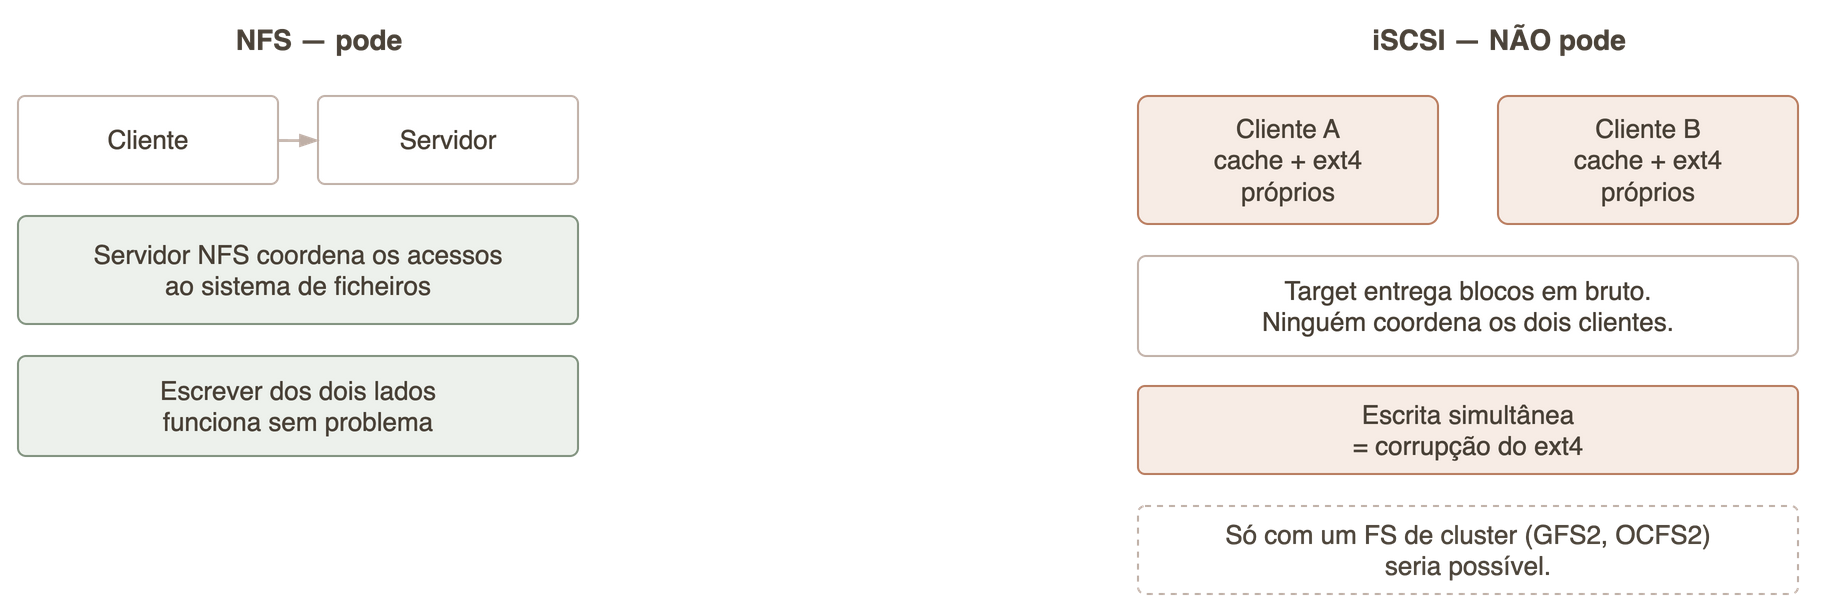
\includegraphics[width=\linewidth]{../Diagramas/m11-concorrencia.png}\\[0.15cm]
{\small\color{NudeTaupe} A diferença que distingue armazenamento de ficheiro de armazenamento de bloco.}
\end{center}


Monte a mesma partilha \textbf{também no servidor}, num ponto diferente:

\textbf{[SRV]}
\begin{terminal}
$ sudo mkdir -p /mnt/nfs-local
$ sudo mount <IP-do-servidor>:/srv/nfs/partilha /mnt/nfs-local
\end{terminal}

Agora escreva dos dois lados alternadamente:

\textbf{[CLI]}
\begin{terminal}
$ echo "linha escrita pelo cliente" | sudo tee /mnt/nfs/concorrente.txt
\end{terminal}

\textbf{[SRV]}
\begin{terminal}
$ cat /mnt/nfs-local/concorrente.txt
$ echo "linha acrescentada pelo servidor" | sudo tee -a /mnt/nfs-local/concorrente.txt
\end{terminal}

\textbf{[CLI]}
\begin{terminal}
$ cat /mnt/nfs/concorrente.txt
\end{terminal}

\begin{saida}
linha escrita pelo cliente
linha acrescentada pelo servidor
\end{saida}

\begin{verificar}
\textbf{Funcionou.} Ambos os lados veem as alterações um do outro, sem corrupção. Porquê? Porque é o \emph{servidor NFS} que gere o sistema de ficheiros e coordena os acessos. Guarde esta observação -- vamos contrastá-la já a seguir.
\end{verificar}

\section{Parte C -- iSCSI: armazenamento ao nível de bloco}

\subsection{Criar o disco virtual}

\textbf{[SRV]}
\begin{terminal}
$ sudo mkdir -p /srv/iscsi
$ sudo truncate -s 500M /srv/iscsi/disco0.img
$ ls -lh /srv/iscsi/
\end{terminal}

\subsection{Configurar o target}

\textbf{[SRV]}
\begin{terminal}
$ sudo targetcli
\end{terminal}

Dentro da consola do \texttt{targetcli}, escreva cada linha:
\begin{terminal}
/> backstores/fileio create disco0 /srv/iscsi/disco0.img
/> iscsi/ create iqn.2026-11.icn.estga:servidor
/> iscsi/iqn.2026-11.icn.estga:servidor/tpg1/luns create /backstores/fileio/disco0
/> iscsi/iqn.2026-11.icn.estga:servidor/tpg1/acls create iqn.2026-11.icn.estga:cliente
/> saveconfig
/> exit
\end{terminal}

\begin{nota}
Traduzindo: criámos um \emph{backstore} (o ficheiro que serve de disco), um \emph{target} identificado por um IQN, uma \emph{LUN} (a unidade que o cliente verá) e uma \emph{ACL} que autoriza um cliente específico, também identificado por IQN.
\end{nota}

\begin{atencao}
Os IQNs do ACL (no servidor) e do initiator (no cliente) \textbf{têm de coincidir exatamente}. É aqui que a maioria dos erros acontece. Copie com cuidado.
\end{atencao}

\subsection{Configurar o cliente}

\textbf{[CLI]}
\begin{terminal}
$ sudo nano /etc/iscsi/initiatorname.iscsi
\end{terminal}

Substitua a linha existente por:
\begin{terminal}
InitiatorName=iqn.2026-11.icn.estga:cliente
\end{terminal}

\textbf{[CLI]}
\begin{terminal}
$ sudo systemctl restart iscsid open-iscsi
$ sudo iscsiadm -m discovery -t sendtargets -p <IP-do-servidor>
\end{terminal}

\begin{saida}
192.168.1.50:3260,1 iqn.2026-11.icn.estga:servidor
\end{saida}

\begin{terminal}
$ sudo iscsiadm -m node --targetname iqn.2026-11.icn.estga:servidor --login
\end{terminal}

\begin{saida}
Login to [iface: default, target: iqn.2026-11.icn.estga:servidor, portal: ...] successful.
\end{saida}

\subsection{Usar o disco}

\textbf{[CLI]}
\begin{terminal}
$ lsblk
\end{terminal}

Procure um disco novo de 500M (ex.\ \texttt{sdb}).

\begin{atencao}
Confirme bem qual é o disco novo antes do próximo comando. Formatar o disco errado destrói a VM.
\end{atencao}

\textbf{[CLI]}
\begin{terminal}
$ sudo mkfs.ext4 /dev/sdX
$ sudo mkdir -p /mnt/iscsi
$ sudo mount /dev/sdX /mnt/iscsi
$ echo "ola via iscsi" | sudo tee /mnt/iscsi/teste.txt
$ df -h /mnt/iscsi
\end{terminal}

\begin{verificar}
Repare no que teve de fazer que \textbf{não} fez no NFS: \textbf{formatar}. Recebeu um dispositivo de bloco em bruto, e foi o \emph{cliente} que lhe criou um sistema de ficheiros.
\end{verificar}

\subsection{Porque não pode partilhar este LUN}

\begin{atencao}
\textbf{Não faça isto:} montar este mesmo LUN em escrita a partir de um segundo cliente ao mesmo tempo.

No NFS funcionou porque o servidor coordena os acessos. No iSCSI não há coordenação nenhuma: cada cliente teria a sua própria cache e as suas próprias estruturas de ext4 em memória, sem saber da existência do outro. O resultado seria a corrupção do sistema de ficheiros.

Para permitir escrita simultânea sobre um dispositivo de bloco partilhado seria necessário um \textbf{sistema de ficheiros de cluster} (GFS2, OCFS2), com bloqueio distribuído.
\end{atencao}

\begin{center}
\begin{tabular}{@{}lll@{}}
\toprule
 & \textbf{NFS (ficheiro)} & \textbf{iSCSI (bloco)} \\
\midrule
O que o cliente recebe & Uma pasta & Um disco em bruto \\
Quem formata & Já estava formatado & O cliente \\
Quem gere o FS & O servidor & O cliente \\
Vários clientes a escrever & Sim & Não (sem FS de cluster) \\
\bottomrule
\end{tabular}
\end{center}

\section{Parte D -- Object storage com MinIO}

\textbf{[SRV]}
\begin{terminal}
$ sudo mkdir -p /srv/minio-data
$ docker run -d --name minio -p 9000:9000 -p 9001:9001 \
    -e "MINIO_ROOT_USER=admin" \
    -e "MINIO_ROOT_PASSWORD=minioadmin123" \
    -v /srv/minio-data:/data \
    minio/minio server /data --console-address ":9001"
$ docker ps | grep minio
\end{terminal}

Abra a consola web em \texttt{http://<IP-do-servidor>:9001}.

\subsection{Cliente \texttt{mc}}

\textbf{[SRV]}
\begin{terminal}
$ curl -O https://dl.min.io/client/mc/release/linux-amd64/mc
$ chmod +x mc
$ ./mc alias set localminio http://localhost:9000 admin minioadmin123
\end{terminal}

\subsection{Bucket e objetos}

\begin{terminal}
$ ./mc mb localminio/dados-aula11
$ echo "objeto de teste" > objeto.txt
$ ./mc cp objeto.txt localminio/dados-aula11/objeto.txt
$ ./mc ls localminio/dados-aula11
$ ./mc cp localminio/dados-aula11/objeto.txt objeto-descarregado.txt
$ cat objeto-descarregado.txt
\end{terminal}

\begin{verificar}
Não montou nada. Não formatou nada. O acesso foi por \textbf{API HTTP} -- um modelo completamente diferente dos dois anteriores.
\end{verificar}

Confirme que o objeto é apenas um ficheiro no servidor:
\begin{terminal}
$ sudo ls -R /srv/minio-data/
\end{terminal}

\section{Parte E -- NFS como PersistentVolume (opcional)}

Requer o cluster da Aula 05.

Instale o cliente NFS em \textbf{todos os nós}:
\begin{terminal}
$ sudo apt install -y nfs-common
\end{terminal}

Crie e aplique o \texttt{nfs-pv.yaml} do Guião 11:
\begin{terminal}
$ kubectl apply -f nfs-pv.yaml
$ kubectl get pv,pvc
\end{terminal}

\begin{saida}
NAME     CAPACITY   ACCESS MODES   STATUS   CLAIM
nfs-pv   1Gi        RWX            Bound    default/nfs-pvc
\end{saida}

\begin{nota}
\texttt{RWX} é \texttt{ReadWriteMany} -- vários nós podem escrever ao mesmo tempo. Só é possível porque o NFS é armazenamento \emph{ao nível de ficheiro}. Com iSCSI teria de usar \texttt{ReadWriteOnce}, pela razão que viu na Parte C.
\end{nota}

Crie os dois Pods do guião e confirme:
\begin{terminal}
$ kubectl exec leitor -- cat /dados/k8s.txt
\end{terminal}

E no servidor NFS:
\begin{terminal}
$ cat /srv/nfs/partilha/k8s.txt
\end{terminal}

\section{Limpeza}

\textbf{[CLI]}
\begin{terminal}
$ sudo umount /mnt/iscsi
$ sudo iscsiadm -m node --targetname iqn.2026-11.icn.estga:servidor --logout
$ sudo umount /mnt/nfs
\end{terminal}

\textbf{[SRV]}
\begin{terminal}
$ sudo umount /mnt/nfs-local
$ docker rm -f minio
\end{terminal}

\section{Problemas frequentes}

\problema{\texttt{mount.nfs: access denied by server while mounting}}
O IP do cliente não está abrangido pela sub-rede em \texttt{/etc/exports}. Confirme o IP real do cliente e a sub-rede que escreveu. Depois de corrigir: \texttt{sudo exportfs -ra}.

\problema{\texttt{mount.nfs: Connection timed out}}
O servidor NFS não está a correr, ou há firewall pelo meio. Teste:
\begin{terminal}
$ sudo systemctl status nfs-kernel-server
$ showmount -e <IP-do-servidor>
\end{terminal}

\problema{Escrevo no NFS mas dá \texttt{Permission denied}}
Problema de permissões ou de mapeamento de UIDs. Para efeitos de laboratório, o \texttt{chmod 777} da secção 2.1 resolve. Em produção usar-se-ia consistência de UIDs ou Kerberos.

\problema{\texttt{iscsiadm: No portals found}}
O target não está a correr ou o IP está errado. No servidor:
\begin{terminal}
$ sudo systemctl status rtslib-fb-targetctl
$ sudo targetcli ls
\end{terminal}

\problema{Erro 24 no \texttt{iscsiadm}: \emph{iSCSI login failed due to authorization failure}}
Os IQNs não coincidem. Compare exatamente:
\begin{terminal}
# no cliente:
$ cat /etc/iscsi/initiatorname.iscsi
# no servidor:
$ sudo targetcli ls /iscsi/iqn.2026-11.icn.estga:servidor/tpg1/acls
\end{terminal}

\problema{O disco iSCSI não aparece no \texttt{lsblk} depois do login}
Aguarde alguns segundos e repita. Se persistir, force a deteção:
\begin{terminal}
$ sudo iscsiadm -m session --rescan
\end{terminal}

\problema{A configuração do targetcli desaparece após reiniciar}
Faltou o \texttt{saveconfig}. Volte a entrar no \texttt{targetcli} e execute-o.

\problema{O MinIO não arranca}
Veja os logs:
\begin{terminal}
$ docker logs minio
\end{terminal}
A password tem de ter pelo menos 8 caracteres -- é um requisito do MinIO.

\problema{\texttt{./mc: Permission denied}}
Faltou o \texttt{chmod +x mc}.

\problema{O PVC fica em \texttt{Pending}}
O PV e o PVC têm de ter modos de acesso e capacidade compatíveis, e o PVC precisa de \texttt{storageClassName: ""} para ligar a um PV estático. Investigue:
\begin{terminal}
$ kubectl describe pvc nfs-pvc
\end{terminal}

\section{Referência rápida}

\begin{center}
\begin{tabular}{@{}ll@{}}
\toprule
\textbf{Comando} & \textbf{Para que serve} \\
\midrule
\texttt{sudo exportfs -ra} & Reaplicar as exportações NFS \\
\texttt{sudo exportfs -v} & Ver o que está exportado \\
\texttt{showmount -e <ip>} & Ver exportações de um servidor \\
\texttt{mount <ip>:/caminho /mnt/x} & Montar partilha NFS \\
\midrule
\texttt{sudo targetcli} & Configurar targets iSCSI \\
\texttt{targetcli ls} & Ver a configuração atual \\
\texttt{iscsiadm -m discovery -t sendtargets -p <ip>} & Descobrir targets \\
\texttt{iscsiadm -m node -{}-targetname X -{}-login} & Ligar a um target \\
\texttt{iscsiadm -m session} & Ver sessões ativas \\
\midrule
\texttt{mc alias set NOME URL user pass} & Configurar acesso ao MinIO \\
\texttt{mc mb alias/bucket} & Criar bucket \\
\texttt{mc cp origem destino} & Copiar objetos \\
\texttt{mc ls alias/bucket} & Listar conteúdo \\
\bottomrule
\end{tabular}
\end{center}

\section{Checklist final}

\begin{itemize}
  \item[$\square$] Identifiquei os tipos de storage de rede suportados pelo Proxmox
  \item[$\square$] Sei explicar a relação entre storage partilhado e migração ao vivo
  \item[$\square$] Configurei o NFS e montei a partilha no cliente
  \item[$\square$] \textbf{Testei o acesso concorrente ao NFS com sucesso}
  \item[$\square$] Configurei o target iSCSI e liguei-me a partir do initiator
  \item[$\square$] Formatei e montei o disco iSCSI, e percebo porque foi preciso formatar
  \item[$\square$] Sei explicar porque não posso partilhar o LUN iSCSI entre dois clientes
  \item[$\square$] Corri o MinIO, criei um bucket e enviei/obtive um objeto
  \item[$\square$] (Opcional) Criei o PV NFS no Kubernetes e percebo o \texttt{ReadWriteMany}
  \item[$\square$] Desmontei tudo e removi o container do MinIO
\end{itemize}

\end{document}
